\chapter{Connecting Morse Theory and Persistence Computations}
\label{ch:connection}
This chapter is dedicated to the connection between discrete Morse functions and persistent homology computations, which in general is a popular consideration. See \cite{MorseTheoryForFiltrations} for an example of how Morse theory can be used to simplify persistent homology computations. 

We will consider some direct translations between filtrations and discrete Morse functions and will try to answer the question if and how \enquote{complex} Morse functions translate to filtrations with expensive persistent homology computations. Looking into this was motivated by talks with Frank Lutz and $\text{Pawe\l}$ $\text{D\l otko}$, who suggested that this connection might be interesting to explore.

\section{Discrete Morse Functions and Filtrations}
We will begin by considering some insights Ulrich Bauer has recently discussed in \cite{bauer2019ripser}. The definition of \textbf{apparent pairs}, the first two lemmas regarding this notion and their respective proofs follow \cite{bauer2019ripser} closely. Afterwards we will build on and extend this theory. Algorithm \ref{algo:filtration_to_dmf} is a straight forward approach and Algorithm \ref{algo:dmf_to_filtration} was suggested by $\text{Pawe\l}$ $\text{D\l otko}$. The lemmas concerned with the relation of these algorithms, namely Lemma \ref{lemma:vector_field_apparent_pairs} and Lemma \ref{lemma:inclusion_of_critical_sets}, were developed for this thesis.

\begin{defi}
Let $K$ be a simplicial complex and let $F_*$ be a simplexwise filtration of $K$. We call a pair $(\sigma,\tau)$ of simplices in $K$ an \textbf{apparent pair} if the following holds
\begin{itemize}
    \item $\sigma$ is the youngest facet of $\tau$,
    \item $\tau$ is the oldest cofacet of $\sigma$.
\end{itemize}{}
\end{defi}

Here, \textbf{young} means, coming late in the filtration and \textbf{old} means coming early in the filtration. Consider the simplexwise filtration of the simplicial complex of a triangle with all its faces. In this chapter, we will label vertices by $0$ to number of vertices. With respect to a triangle this means we label the vertices $0$, $1$ and $2$, and therefore get the following filtration for the simplicial complex of a $2$-simplex: \[
    F_* = ([0],[1],[2],[0,1],[0,2],[1,2],[0,1,2]).
\]
The youngest facet of the edge $[0,1]$ is the vertex $[1]$ and the oldest cofacet of vertex $[1]$ is the edge $[0,1]$. Hence $([1],[0,1])$ is an apparent pair. 
Consider the boundary matrix of this example, in which we have highlighted the lowest $1$s in each column by a gray box:
\[
\begin{blockarray}{cccccccc}
& [0] & [1] & [2] & [0,1] & [0,2] & [1,2] & [0,1,2]  \\
\begin{block}{c[ccccccc]}
  [0] & 0 & 0 & 0 & 1 & 1 & 0 & 0\\*
  \left[1\right] & 0 & 0 & 0 & \colorbox{lightgray}{1} & 0 & 1 & 0\\*
  \left[2\right] & 0 & 0 & 0  & 0 & \colorbox{lightgray}{1} &\colorbox{lightgray}{1} & 0\\*
  \left[0,1\right] & 0 & 0 & 0  & 0 & 0 & 0 & 1 \\*
  \left[0,2\right] & 0 & 0 & 0  & 0 & 0 & 0 & 1\\*
  \left[1,2\right] & 0 & 0 & 0  & 0 & 0 & 0 & \colorbox{lightgray}{1}\\*
\end{block}
\end{blockarray}
\]
As we can see in this case, all three apparent pairs are also persistence pairs, since the respective columns are already reduced and have their lowest $1$s in the rows corresponding to the other element of the apparent pair. This generally holds true.
\begin{lemma}
\label{lem:app_is_pers}
An apparent pair of a simplexwise filtration is a persistence pair.
\end{lemma}
\begin{proof}
Let $K$ be a simplicial complex. Let $F_*$ be a simplexwise filtration of $K$ and let $B$ be its boundary matrix. Consider an apparent pair $(\sigma, \tau)$ of~$F_*$. 

Assume $\beta \neq \sigma$ is the row with the lowest $1$ in column $\tau$. Then $\beta$ is a facet of $\tau$ coming later in the filtration than $\sigma$. This contradicts $(\sigma, \tau)$ being an apparent pair. Similarly assume there is another column to the left of $\tau$, which has a non-zero entry in row $\sigma$. This means, that $\tau$ is not the oldest cofacet of $\sigma$. 

Again this contradicts $(\sigma, \tau)$ being an apparent pair.
 
Hence column $\tau$ is already reduced and by the pairing lemma it follows that  $(\sigma, \tau)$ is a persistence pair. 
\end{proof}

Furthermore the set of apparent pairs is a discrete gradient on $K$.

\begin{lemma}
The apparent pairs of a simplexwise filtration $F_* = (\sigma_0, \dots, \sigma_m)$ form a gradient vector field.
\label{lemma:apparent_pairs_form_gradient}
\end{lemma}
\begin{proof}
The proof will be done in two steps. First we prove, that the apparent pairs form a discrete vector field. Then we define a Morse function that has the apparent pairs as gradient pairs. 

Let $(\sigma^{(k)}, \tau^{(k+1)})$ be an apparent pair. Since $\tau$ is uniquely determined by $\sigma$, there can be no other apparent pair $(\sigma^{(k)}, \xi^{(k+1)})$ that contains $\sigma$. We will show that there can also be no apparent pair $(\phi^{(k-1)},\sigma^{(k)})$ containing~$\sigma$. Note that in this case $k \geq 1$. There is another $k$-simplex $\rho \neq \sigma$ that is a facet of $\tau$ and a cofacet of $\phi$. By assumption $\sigma$ is the youngest facet of $\tau$, hence $\rho$ is older than $\sigma$. In particular $\sigma$ is not the oldest cofacet of $\rho$ and hence $(\rho,\sigma)$ is not an apparent pair. 
An analogous argument shows that $\tau$ also can not be in another apparent pair. Therefore the apparent pairs form a discrete vector field. 

We will now show that the apparent pairs are the gradient pairs of a Morse function. Recall $F_* = (\sigma_0, \dots, \sigma_m)$ and define
\[
f(\sigma_j)= \begin{cases} 
      i & \text{if there is an apparent pair$(\sigma_i,\sigma_j)$}, \\
      j & \text{else.} 
   \end{cases}
\]

We will verify that $f$ is a Morse function. It holds that $f(\sigma_l) \leq l$. Furthermore let $\sigma_i$ be a facet of $\sigma_l$, i.e., $i<j$. If $(\sigma_i, \sigma_j)$ is not an apparent pair then $f(\sigma_i)\leq i < j = f(\sigma_j)$. In particular $(\sigma_i, \sigma_j)$ is not a gradient pair of $f$. 

Now assume $(\sigma_i, \sigma_j)$ is an apparent pair, i.e., $\sigma_i$ is the youngest facet of $\sigma_j$. Then we have $h \leq i$ for every $\sigma_h$ that is a facet of $\sigma_j$. Thus $f(\sigma_h) \leq h \leq i = f(\sigma_j)$, where equality holds if and only if $h = i$. Meaning, there is exactly one facet of $\sigma_j$, namely $\sigma_i$, with function value not lower than $f(\sigma_j)$. Hence $f$ is a Morse function and the gradient pairs of $f$ are the apparent pairs of the filtration $F_*$.

\end{proof}

We will also refer to this discrete gradient field as the \textbf{apparent gradient} of $F_*$. As with discrete vector fields we will call the lower dimensional element of an apparent pair its \textbf{tail} and the higher dimensional element its \textbf{head}. Note that from the proof we also get a definition for a Morse function, that has the pairs of the apparent gradient as gradient pairs.

The following example illustrates that the apparent gradient does not necessarily yield an optimal Morse matching. Consider the filtration \[
F_* = ([0],[1],[2],[3],[4],[5],[4,5],[2,3],[0,1],[1,2],[3,5],[0,4]).
\]
Figure \ref{fig:not_opt_example} shows a possible geometric realization and the apparent gradient of $F_*$. There are three critical cells and we know the induced Morse matching is not optimal since we can also match $[2]$ and $[1,2]$ as well as $[4]$ and $[0,4]$ without closing a $V$-path. Indeed adding these pairs yields a perfect Morse matching.


\begin{figure}[H]
\noindent%
\centering%
\begin{tikzpicture}

\node[b_circle, name path=0, label=above:{0}] (0) at (0,4) {};

\node[b_circle, name path=1, label=left:{1}] (1) at (-2,2) {};

\node[b_circle, name path=1, label=right:{4}] (4) at (2,2) {};

\node[b_circle, name path=1, label=left:{2}] (2) at (-2,0) {};

\node[b_circle, name path=1, label=right:{5}] (5) at (2,0) {};

\node[b_circle, name path=1, label=below:{3}] (3) at (0,-2) {};


\draw[thick] (0) to (4);
\draw[thick] (3) to (5);
\draw[thick] (1) to (2);
\draw[->-, very thick] (1) to (0);
\draw[->-, very thick] (3) to (2);
\draw[->-, very thick] (5) to (4);


\end{tikzpicture}

\caption{Geometric realization of the simplicial complex of $F_*$ and its apparent gradient.}
\label{fig:not_opt_example}

\end{figure}


A simple algorithmic approach to construct this gradient vector field is to iterate over all simplices in a simplexwise filtration in order of appearance and for each element search for the youngest facet, then check if the current element is that facets oldest cofacet.\\ The following algorithm does exactly that while keeping track of all critical faces.

\begin{algorithm}[H]
\SetKwData{Left}{left}\SetKwData{This}{this}\SetKwData{Up}{up}\SetKwFunction{Union}{Union}\SetKwFunction{FindCompress}{FindCompress}\SetKwInOut{Input}{Input}\SetKwInOut{Output}{Output}
\Input{Filtration $F_* = (\sigma_1, ..., \sigma_m)$, simplicial complex $K$}
\Output{Discrete gradient $V$, Critical cells $C$}

Initialize $C$ as the set of vertices and $V$ as the empty set\\
\For{$\sigma \in F$ in order of appearance}
{
    $\gamma = $ youngest facet of $\sigma$\\
    \If{$\sigma$ oldest cofacet of $\gamma$}
    {Add $(\sigma,\gamma)$ to $V$, remove $\gamma$ from $C$}
    \Else{Add $\sigma$ to $C$}
}

$\operatorname{return}(V,C)$
\caption{Filtration to discrete gradient field.}

\label{algo:filtration_to_dmf}
\end{algorithm} 
\vspace{0.5cm}

Note that simplices are added to the set of critical cells and removed later on, if they are paired with a cofacet. 

The outer loop starting in Line 2 runs in $\mathcal{O}(m)$, where $m$ is the number of simplices in the filtration. At the time of considering $\sigma$ there are two possibilities.

Either its youngest facet $\gamma$ is not already paired and $\sigma$ is the oldest cofacet of $\gamma$. See Line 4. In this case we pair $\sigma$ and $\gamma$ and remove $\gamma$ from the set of critical simplices. 

Or the condition is not fulfilled. This causes $\sigma$ to be declared critical for now.

Checking the conditions is in $\mathcal{O}(m)$ each, and assuming that adding and removing elements from $V$ and $C$ takes constant time we get overall quadratic running time in the number of simplices of the filtration.

At the end of the algorithm all simplices remaining in the set $C$ are critical and all others are part of an apparent pair.

Applying this algorithm to the filtration \[
   F_* = ([0],[1],[2],[0,1],[0,2],[1,2],[0,1,2]).
\]
yields the discrete vector field depicted in Figure \ref{fig:algo1_example}. 

\begin{figure}[H]
\noindent%
%\centering%

\centering%
\begin{tikzpicture}

\node[b_circle, name path=0, label=below:{0}] (0) at (0,0) {};

\node[b_circle, name path=1, label=below:{1}] (1) at (2,0) {};

\node[b_circle, name path=2, label=above:{2}] (2) at  (1,2) {};


\draw[thick] (2) to (1);
\draw[->-, thick] (1) to (0);

\draw[->-, thick] (2) to (0);
\draw[->, thick] (1.5,1) to (1,0.75);

\fill[opacity = 0.2] (0,0) -- (2,0) -- (1,2);

\end{tikzpicture}

\caption{A simplicial complex with discrete gradient}
\label{fig:algo1_example}

\end{figure}


A natural question is, how to invert this process, i.e., how to get from a discrete gradient to a filtration in which the pairs of the gradient correspond to apparent pairs.

Recall the modified Hasse diagram from the last chapter. The modified Hasse diagram of the simplicial complex and discrete Morse function from Figure \ref{fig:algo1_example} is depicted in the following Figure \ref{fig:modified_hasse}. 

\begin{figure}[H]
\noindent%
%\centering%
\centering%
\begin{tikzpicture}

\node[circle, name path=0, label=below:{[0]}] (0) at (-1.5,0) {};
\node[circle, name path=1, label=below:{[1]}] (1) at (0,0) {};
\node[circle, name path=2, label=below:{[2]}] (2) at  (1.5,0) {};

\node[circle, name path=0, label=left:{[0,1]}] (3) at (-1.5,1.5) {};
\node[circle, name path=1, label=right:{[0,2]}] (4) at (0,1.5) {};
\node[circle, name path=2, label=right:{[1,2]}] (5) at  (1.5,1.5) {};

\node[circle, name path=1, label=above:{[0,1,2]}] (6) at (0,3) {};

\draw[->, thick] (5) to (6);
\draw[->, thick] (6) to (3);
\draw[->, thick] (6) to (4);

\draw[->, thick] (3) to (0);
\draw[->, thick] (4) to (0);

\draw[->, thick] (5) to (1);
\draw[->, thick] (1) to (3);

\draw[->, thick] (2) to (4);
\draw[->, thick] (5) to (2);

\end{tikzpicture}
\caption{The modified Hasse diagram of the previously seen complex and discrete vector field.}
\label{fig:modified_hasse}
\end{figure}


The following algorithm to obtain a simplexwise filtration from a discrete vector field $V$ and a simplicial complex $K$ was suggested by $\text{Pawe\l}$ $\text{D\l otko}$. We assume the reader is familiar with topological sorting. 

In the version of it we are using, the set of all elements is partitioned such that the first set has no dependencies, the elements of the second set depend on the first etc. Within these sets we will order the elements lexicographically. 

Note that the usual convention regarding topological sorting is, that a directed edge from some node $a$ to some node $b$ implies $a \prec b$. In our case it is the other way around. 


\begin{algorithm}[H]
\SetKwData{Left}{left}\SetKwData{This}{this}\SetKwData{Up}{up}\SetKwFunction{Union}{Union}\SetKwFunction{FindCompress}{FindCompress}\SetKwInOut{Input}{Input}\SetKwInOut{Output}{Output}
\Input{Simplicial complex $K$, Discrete gradient field $V$}
\Output{Simplexwise filtration $F_*$}

$H_K^V =$ modified Hasse diagram of $K$ and $V$\\
$Filtration = $ topological sorting of $(H_K^V)$\\
Sort $Filtration$ by dimension in a stable manner.\\
$\operatorname{return}(Filtration)$
\caption{Discrete gradient field to filtration}
\label{algo:dmf_to_filtration}
\end{algorithm} 
\vspace{0.5cm}

By sorting the simplices by dimension in Line 3 we are guaranteed to get a valid simplexwise filtration. Sorting in a stable manner means, that two elements of the same size, i.e. dimension, remain in the same internal order as before. 

This algorithm only generates filtrations that are ordered by dimension which is quite restrictive in a sense. If we are mainly interested in the number of reduction steps needed to reduce the corresponding boundary matrix, however, this is no restriction at all. Any filtration $F$ and a filtration~$F'$ which is equal to $F$ sorted by dimension in a stable manner, yield the same persistence pairs and need their boundary matrices to be reduced by the same steps. 


For an example of the algorithm consider the modified Hasse diagram of Figure \ref{fig:modified_hasse}. The topological ordering we get in line 2 is
\[
     ([0], [0,1], [0,2], [0,1,2], [1], [2], [1,2]).
\]
At this point we do not have a valid filtration. But after the algorithm executes Line 3, in which we sort by dimension, while keeping the order within the dimensions intact, we get 
\begin{center}
$F_* = ([0],[1],[2],[0,1],[0,2],[1,2],[0,1,2])$.
\end{center} 

We will now formally describe in which way the two Algorithms~\ref{algo:filtration_to_dmf}~and~ \ref{algo:dmf_to_filtration} are inverse to one another. We will write $F_* = \mathcal{F}(V)$ for the filtration that is generated by the discrete vector field $V$ in Algorithm \ref{algo:dmf_to_filtration}. For brevity, we will omit a reference to the underlying simplicial complex $K$. Conversly we write $V = \mathcal{V}(F)$ for the gradient vector field generated by Algorithm \ref{algo:filtration_to_dmf}.
The following Lemma proves that Algorithm \ref{algo:dmf_to_filtration} generates a filtration with the desired properties. 

\begin{lemma}
Let $V$ be a gradient vector field on simplicial complex $K$ and let $F_* = \mathcal{F}(V)$ be the generated filtration. Every pair in $V$ is an apparent pair in $F_*$. 
\label{lemma:vector_field_apparent_pairs}
\end{lemma}
\begin{proof}
Let $(\sigma^{(p-1)},\tau^{(p)})$ be a pair in $V$. Recall that, by definition, $\tau$ and $\sigma$ can not be part of any other pair. Now consider $H_K^V$, the modified Hasse diagram of $K$ and $V$. Let $\gamma$ be a facet of $\tau$, with $\gamma \neq \sigma$.

In $H_K^V$, $\tau$ has a directed edge to $\gamma$, since $(\gamma,\tau)$ is not a pair in $V$. But $\sigma$ has a directed edge to its cofacet $\tau$, since $(\sigma,\tau)$ is a pair in $V$, so in $H_K^V$ we get a directed edge from $\sigma$ to $\tau$ and therefore a directed path from $\sigma$ to $\gamma$. Hence, in the topological order $\gamma \prec \sigma$ and therefore in the filtration every such $\gamma$ comes before $\sigma$. It follows that $\sigma$ is the youngest facet of $\tau$. 

Analogously, let $\theta$ be a cofacet of $\sigma$, $\theta \neq \tau$. Now in $H_K^V$ we have a directed edge from $\sigma$ to  $\tau$ and another directed edge from $\theta$ to $\sigma$. Again it follows, that $\tau \prec \theta$, meaning that $\tau$ is the oldest cofacet of $\sigma$. 

The pair $(\sigma,\tau) \in V$ was chosen arbitrarily, hence the claim follows. 
\end{proof}

\begin{lemma}
Let $V_0$ be a discrete vector field and let $C_0$ be the set of critical cells of $V_0$. Now let $V_1 = \mathcal{V}(\mathcal{F}(V_0))$ be the discrete vector field generated by concatenating the respective algorithms. Let $C_1$ be the set of critical cells of~$V_1$. Then $C_1 \subseteq C_0$.
\label{lemma:inclusion_of_critical_sets}
\end{lemma}
\begin{proof}
By Lemma \ref{lemma:vector_field_apparent_pairs}, every pair in $V_1$ is an apparent pair in $\mathcal{F}(V_1)$, which again, is a pair in $ V_2 = \mathcal{V}(\mathcal{F}(V_1))$ by Lemma \ref{lemma:apparent_pairs_form_gradient}. Since every simplex that is not part of a pair, is critical, the claim follows. 
\end{proof}

\begin{corl}
Let $V_0$ be a discrete vector field and define $V_i = \mathcal{V}\mathcal{F}((V_{i-1}))$ for $i\in \mathbb{N}$. Then after finitely many steps $k$, we get that $V_k = V_{k-1}$.
\end{corl}
 
This means that after repeatedly applying the algorithms  all apparent pairs of the filtration are pairs in the apparent gradient and vice versa. For an example of an iteration that actually decreases the number of critical cells, consider the simplicial complex from Figure \ref{fig:not_opt_example} again. The corresponding filtration is  \[
F_*^1 = ([0],[1],[2],[3],[4],[5],[4,5],[2,3],[0,1],[1,2],[3,5],[0,4]).
\]
Using $F_*^1$ as input for Algorithm \ref{algo:filtration_to_dmf} yields the apparent gradient \[V_1 = \{([1],[0,1]),([5],[4,5]),([2],[2,3])\}.\] Using $V_1$ and the underlying simplicial complex of $F_*^1$ as input for Algorithm \ref{algo:dmf_to_filtration} yields the filtration \[
F_*^2 = ([0], [2], [4], [1], [3], [5], [0, 1], [0, 4], [2, 3], [4, 5], [1, 2], [3, 5]),
\]
which has apparent gradient \[V_2 = \{([1],[0,1]),([4],[0,4]),([5],[4,5]),([2],[2,3])\}.\] This means the number of critical cells actually decreased and two critical cells remain.

This stabilization process yields altering filtrations and discrete gradients, but we never loose an apparent pair. This means that the filtrations remain close in the sense, that every pair that is an apparent pair once remains a persistence pair in every iteration of the process. Analogously no apparent gradient ever looses a pairing. 

It remains to be uncovered if this relates to other notions of closeness of persistence computations we do not discuss in this work or if there are bounds on how many iterations we have to do until the process stabilizes. 

\section{V-Paths and Standard Reduction}
In this section we will explore relations between $V$-paths of the apparent gradient of a filtration and the number of conflicts in the standard reduction scheme. All lemmas and the theorem discussed in this section are not based on previously known works but were developed for this thesis with guidance by $\text{Pawe\l}$ $\text{D\l otko}$.

Recall Definition \ref{def:col_red_steps}, i.e., the definition of the number of column reduction steps $\operatorname{red}(B)$ during the reduction of some boundary matrix $B$ corresponding to filtration $F_*$. We will now link this to the length of $V$-paths of the apparent gradient of $F_*$.


The following example will provide an intuition for the connection. Consider the following filtration:
\[
    F_* = ([0],[1],[2],[3],[4],[0,1],[0,2], [1,3], [2,4], [1,2], [3,4]).
\]

A geometric realization of the underlying abstract simplicial complex is depicted in the following figure. It also shows the apparent gradient of $F_*$.

\begin{figure}[H]
\noindent%
%\centering%
\centering%
\begin{tikzpicture}

\node[b_circle, name path=0, label=below:{0}] (0) at (4,1) {};

\node[b_circle, name path=1, label=above:{1}] (1) at (2,2) {};
\node[b_circle, name path=2, label=above:{3}] (3) at (0,2) {};

\node[b_circle, name path=1, label=below:{2}] (2) at (2,0) {};
\node[b_circle, name path=2, label=below:{4}] (4) at (0,0) {};


\draw[->-, thick] (1) to (0);
\draw[->-, thick] (3) to (1);

\draw[->-, thick] (2) to (0);
\draw[->-, thick] (4) to (2);

\draw[-, thick] (3) to (4);
\draw[-, thick] (1) to (2);

\end{tikzpicture}
\caption{An example we will use to illustrate the connection between V-Paths and conflicts in the standard reduction scheme}
\label{fig:paths_and_computations}
\end{figure}

The cropped boundary matrix of $F_*$ looks as follows:
\[
\begin{blockarray}{ccccccc}
& [0,1] & [0,2] & [1,3] & [2,4] & [1,2] & [3,4] \\
\begin{block}{c[cccccc]}
             [0] & 1 & 1 & 0 & 0 & 0 & 0 \\*
  \left[1\right] & \colorbox{lightgray}{1} & 0 & 1 & 0 & 1 & 0 \\*
  \left[2\right] & 0 & \colorbox{lightgray}{1}  & 0 & 1 & \colorbox{lightgray}{1}  & 0 \\*
  \left[3\right] & 0 & 0 & \colorbox{lightgray}{1}  & 0 & 0 & 1 \\*
  \left[4\right] & 0 & 0 & 0 & \colorbox{lightgray}{1}  & 0 & \colorbox{lightgray}{1}   \\*
\end{block}
\end{blockarray}
\]

We have highlighted the lowest $1$s in each column with a small gray box. As we can see every column corresponding to the head of an apparent pair is already reduced, i.e., the lowest $1$ is in a row such that no column to the left of it has its lowest $1$ in the same row.

Now lets try to resolve the conflicts. Column $[1,2]$ is reduced by first adding column $[0,2]$ and then column $[0,1]$. This corresponds to following the $V$-paths originating in the facets of edge $[1,2]$ to the critical vertex $[0]$.

Similarly, reducing column $[3,4]$ requires us to add colum $[2,4]$, $[1,3]$, $[0,2]$ and finally $[0,1]$ which again corresponds to following the $V$-paths originating in the facets of edge the $[3,4]$ and ending in the critical vertex $[0]$. \\

We will now generalize this example. 
For some simplexwise filtration $F_* = (\mu_1,\dots,\mu_m)$ on a simplicial complex $K$, we define $f:K \rightarrow \mathbb{R}$ as $f(\mu_i) = i$ and
call $f$ the \textbf{filtration values} of $F_*$. 

Let $V$ be the apparent gradient of $F_*$. We will refer to simplices that are part of a pair in $V$ as \textbf{paired} and to simplices that are not part of a pair in $V$ as \textbf{unpaired}. Consider some $\tau^{(k+1)} \in K$ and let us denote by $\mathcal{P}_\tau$ the set of all $V$-paths originating in a facet of $\tau$ and ending in an unpaired simplex or a simplex that is the head of an apparent pair. We will call them the \textbf{complete facet paths} of $\tau$. 

In the above example the complete facet paths of edge $[1,2]$ are the paths $P_1 = [1],[0,1],[0]$ and $P_2 = [2],[0,2],[0]$, hence we write $\mathcal{P}_{[1,2]} = \{P_1,P_2\}$.
%When discussing the reduction of some boundary matrix we will abuse notation slightly and refer to the column corresponding to some simplex in the boundary matrix, by the simplex itself, i.e., we will refer to the column coresponding to some simplex $\sigma$ as column $\sigma$. Furthermore for two simplices $\sigma$ and $\alpha$ with $f(\sigma)<f(\alpha)$ we will say that row $\sigma$ is \textbf{above} row $\alpha$, and row $\alpha$ is \textbf{below} row $\sigma$. This stems from the fact that the simplex with lowest filtration value corresponds to the first row of the boundary matrix and the simplex with the highest filtration value corresponds to the last row of the boundary matrix.

\begin{lemma}
\label{lem:lowest_apparent}
With $K,F_*,V$ and $f$ as above. Let $\tau$ be an unpaired simplex, and if there are unpaired elements that are the last elements of a path in $\mathcal{P}_\tau$, let $\sigma^{(k)}$ be the one with highest filtration value. If such a $\sigma$, exists it holds that:
\begin{enumerate}[{(}1{)}]
\item During the reduction of column $\tau$, every lowest $1$ with higher filtration value than $\sigma$ is the tail of an apparent pair and an element of a path in~$\mathcal{P}_\tau$.
\item The reduced column $\tau$ is zero or has a lowest $1$ in row $\sigma$ or a row with lower filtration value.
\end{enumerate}

%\item Every one appearing below row $\sigma$ during reduction is part of an apparent pair and an element in a path in $\mathcal{P}_\tau$.

\end{lemma}
\begin{proof}
Initally all ones in column $\tau$ correspond to facets of $\tau$. Let $\alpha$ be the row corresponding to the lowest $1$. If $\alpha = \sigma$, we are done, so let $\alpha \neq \sigma$.
We will show that $\alpha$ has to be the tail of an apparent pair. 

Assume for the sake of contradiction that $\alpha$ is unpaired. Then the trivial path $P = \alpha$ is in $\mathcal{P}_\tau$. This contradicts the assumption that $\sigma$ is the unpaired simplex with highest filtration value that is the last element of a path in $\mathcal{P}_\tau$. 

Therefore $\alpha$ has to be part of an apparent pair. Assume $\alpha$ is the head of an apparent pair. Then $\alpha$ is part of a persistence pair with some lower dimensional simplex and can not be part of a persistence pair with some higher dimensional simplex. This means, no column can have its lowest $1$ in row $\alpha$. In particular, it can never be the lowest $1$ of column $\tau$ during its reduction. This is a contradiction to the assumption that $\alpha$ corresponds to the lowest $1$ in column $\tau$. Hence, $\alpha$ is the tail of an apparent pair $(\alpha, \beta)$. Furthermore, $\alpha$ is an element of all paths in $\mathcal{P}_\tau$ that begin with the sequence $\alpha,\beta$. In particular $\alpha$ is an element of a path in $\mathcal{P}_\tau$.

To reduce the lowest $1$ in row $\alpha$ we have to add column $\beta$. Since $\beta$ is the head of an apparent pair its column is reduced from the beginning. Therefore the new ones appearing in column $\tau$ correspond to facets of $\beta$ and are themselves lower dimensional elements of a path in $\mathcal{P}_\tau$. 

By the same reasoning as before, every lowest $1$ with higher filtration value than row $\sigma$, corresponds to some tail $\alpha_*$ of an apparent pair and all appearing ones correspond to elements in a path of $\mathcal{P}_\tau$. This proves (1). Furthermore, (2) is a direct consequence of (1), since every lowest $1$ that is the tail of an apparent pair is reduced by adding the column of its head. This continues until the column is zero or the lowest $1$ appears in row $\sigma$. Either $\tau$ and $\sigma$ get paired persistence-wise and the lowest $1$ remains in row $\sigma$, or if $\sigma$ is already paired with another column the reduction continues and after the next reduction step the column is zero or has its lowest $1$ in a row with lower filtration value than $\sigma$.
\end{proof}

Consider the example from Figure \ref{fig:paths_and_computations}. Reducing column $[1,2]$ follows along the previously stated paths in  $\mathcal{P}_{[1,2]}$ and reducing column $[3,4]$ follows along the paths $P_1 = [3],[1,3],[1],[0,1],[0]$ and $P_2 = [4],[2,4],[2],[0,2],[0]$. In the next section we will see an example in which we have a lowest $1$ in a row with lower filtration value than the $\sigma$ from the lemma. 

In the following we will prove one-to-one correspondence between lowest $1$s during the reduction of column $\tau$ and a subset of $\mathcal{P}_\tau$. For some simplex $\mu \in K$, we define $\mathcal{P}_\tau^\mu$, as the set of $V$-paths originating in a facet of $\tau$ and ending in $\mu$, and call them the \textbf{facet paths from} $\bm{\tau}$ \textbf{to} $\bm{\mu}$. We define the number of these paths \[
x_\tau^\mu \coloneqq |\mathcal{P}_\tau^\mu|,
\]
to be the \textbf{$\bm{\tau}$-multiplicity of $\bm{\mu}$}. Note that the elements of $\mathcal{P}_\tau^\mu$ are subsequences of the elements of $\mathcal{P}_\tau$. 

When considering the above example and looking at the multiplicities of the vertices with respect to the different edges, we see that even multiplicity implies that the vertex is never a lowest $1$ in the reduction of a column while odd multiplicity implies the opposite. For example consider the reduction of column $[1,2]$. The vertices $[1]$ and $[2]$ both have odd $[1,2]$-multiplicity and appear as lowest $1$s while vertex $[0]$ has even $[1,2]$-multiplicity and does not appear as a lowest $1$.

\begin{lemma}
\label{lem:oddest_ones}
With the same notations and assumptions as in Lemma \ref{lem:lowest_apparent}, i.e., $\tau^{(k+1)}$ an unpaired simplex and if there are unpaired elements that are the last elements of a path in $\mathcal{P}_\tau$, let $\sigma^{(k)}$ be the one with highest filtration value. Assuming such a $\sigma$ exists, let $\mu^{(k)}\in K$ with $f(\mu)>f(\sigma)$. Then the lowest $1$ of column $\tau$ is in row $\mu$ at some point during the reduction if and only if $x_\tau^\mu$ is odd.
\end{lemma}
\begin{proof}
We split the proof into the two directions of the equivalence. Both directions are proven by inductive arguments.

\enquote{$\Rightarrow$}:
We will prove this direction by an induction over the number of appearing lowest $1$s.

Let the initial lowest $1$ be in row $\mu$. Then $\mathcal{P}_\tau^\mu$ contains the single path $P = \mu$, i.e., $x_\tau^\mu$ is odd. Assume this is true for the first $n$ appearing lowest $1$s. We will now show that it is then also true for the next lowest $1$.
 
Consider $\mu$ with $f(\mu) > f(\sigma)$ to be the row that contains the lowest $1$ after $n$ reduction steps. The entry in row $\mu$ changes its value whenever some column corresponding to a cofacet of $\mu$ gets added to column $\tau$. Let $\{\beta_1, \dots ,\beta_l\}$ be all $l$ columns that are added to column $\tau$ during its reduction that change the value in row $\mu$. Since $f(\mu) > f(\sigma)$, we know by Lemma \ref{lem:lowest_apparent} that each of the $\beta_i$ is part of an apparent pair $(\alpha_i, \beta_i)$ and $\alpha_i$ was a lowest $1$ at some previous point in the reduction. Therefore, by assumption, $x_\tau^{\alpha_i}$ is odd. Furthermore $x_\tau^\mu = \sum_{i = 1}^l x_\tau^{\alpha_i}$. 

We have to consider two cases.

Case one: the entry in row $\mu$ of column $\tau$ initally equals one. Then $l$ has to be even for the entry to be one after the first $n$ reduction steps. If $l>0$, $x_\tau^\mu$ is the sum of an even number of odd values. Hence it is odd. If $l=0$, i.e., $\mu$ is a facet of $\tau$ that is reached only by the trivial path $P$ = $\mu$, then $x_\tau^\mu = 1$. 

Case two: the entry in row $\mu$ of column $\tau$ initally equals zero. Then $l$ has to be odd for the entry to be one after the first $n$ reduction steps. Therefore $x_\tau^\mu$ is the sum of an odd number of odd values. Hence it is odd.

\enquote{$\Leftarrow$}: We will prove the claim by induction over $x_\tau^\mu$ and begin with $x_\tau^\mu = 1$. This means we have some path $P = \alpha_0, \beta_0, \dots, \alpha_r, \beta_r, \mu$ with $\alpha_0$ being a facet of $\tau$. This means the entry in row $\alpha_0$ of column $\tau$ initially equals $1$, and by Lemma \ref{lem:lowest_apparent} (2) we know it has to be set to zero at some point. Assume that the entry in row $\alpha_0$ gets set to zero when some column $\xi$ gets added to column $\tau$. By Lemma \ref{lem:lowest_apparent} (1) we know that $\xi$ is part of an apparent pair and a path in $\mathcal{P}_\tau$. This implies there is another path from a facet of $\tau$ to $\mu$ that contains $P$ as a subsequence. This is a contradiction to the assumption $x_\tau^\mu = 1$. Therefore $\alpha_0$ is the lowest $1$ at some point and reducing it creates a $1$ in row $\alpha_1$. By the same reasoning as with $\alpha_0$ we get that $\alpha_1$ has to be a lowest $1$, and following the $V$-path along to $\mu$ yields that it also has to be a lowest $1$ at some point. 

Assume this holds true for $x_\tau^\mu = n$ with $n$ being odd. We will show it is also true for $x_\tau^\mu = n+2$. 

Let $x_\tau^\mu = n+2$ and let $\gamma$ be the simplex with highest filtration value in which paths in $\mathcal{P}_\tau^\mu$ intersect that are not equal on at least one apparent pair of which the tail has higher filtration value than $\gamma$. This means we are considering paths that might or might not originate in the same facet of $\tau$, are not equal at some point and then intersect (again) in simplex $\gamma$. Note that it is possible that $\gamma = \mu$.

Let $P$ and $Q$ be two of these paths. Assume $Q$ and $P$ are initially the same sequence $\alpha_0,\beta_0, \dots, \alpha_l,\beta_l$. By the assumptions on $\gamma$, there can be no other path in $\mathcal{P}_\tau^\mu$ intersecting this sequence. Therefore by the same reasoning as for the case $x_\tau^\mu = 1$ at some point column  $\beta_l$ gets added to column $\tau$ and the rows corresponding to the first distinct elements of $Q$ and $P$ get set to $1$. Let us denote these sequences by $Q' = \omega_1, \xi_1, \dots, \omega_y, \xi_y, \gamma$ and $P' = \theta_1, \psi_1, \dots, \theta_z, \psi_z, \gamma$. As neither $Q'$ nor $P'$ get intersected due to the assumptions on $\gamma$, we know that at some point of the reduction columns $\xi_y$ and $\psi_z$ get added to column $\tau$. The first addition causes the entry in row $\gamma$ of column $\tau$ to be set to $1$. The second one causes it to be set to $0$. This means that $Q$ and $P$ have no influence on whether there is a lowest $1$ in row $\mu$ at some point. Hence $\mu$ being a lowest $1$ depends on the odd $n$ other paths in $\mathcal{P}_\tau^\mu$, which, by the induction assumption, tells us that $\mu$ indeed is a lowest $1$ at some point.
\end{proof}

With this we also know how lowest $1$s appear with respect to $V$-paths originating in a facet of $\tau$. Again assuming the existence of unpaired last elements of a path in $\mathcal{P}_\tau$ we choose $\sigma$ to be the one with highest filtration value and define: \[
\mathcal{O}_\tau^\sigma \coloneqq \{(\alpha, \beta) \in V \mid f(\alpha) > f(\sigma), \, x_\tau^\alpha \operatorname{mod} 2 = 1 \},
\]
the \textbf{odd pairs} between $\sigma$ and $\tau$. 

\begin{thm}
\label{thm:vpath_delta}
Let $F_*,K,V$, and $f$ be defined as above. Let $\tau^{(k+1)}\in K$ be a simplex that is either not part of an apparent pair or the tail of an apparent pair. If there is an unpaired cell that is the last element of a path in $\mathcal{P}_\tau$, let $\sigma$ be the one with highest filtration value. If $\sigma$ exists, then:
\[
    \operatorname{red}(\tau) \geq |\mathcal{O}_\tau^\sigma|,
\]
with equality holding if $\tau$ and $\sigma$ are a persistence pair or if column $\tau$ gets reduced to zero.
\end{thm}
\begin{proof}
By Lemma \ref{lem:lowest_apparent} (2) we know that every lowest $1$ in column $\tau$ must be reduced until column $\tau$ is zero or has a lowest $1$ in row $\sigma$. By Lemma \ref{lem:oddest_ones} we know that each lowest $1$ corresponds to an element in $\mathcal{O}_\tau^\sigma$. If $\sigma$ is not yet part of a persistence pair or column $\tau$ is reduced to zero, we get that $\operatorname{red}(\tau) = |\mathcal{O}_\tau^\sigma|$. If $\sigma$ is part of a persistence pair, the reduction continues and $\operatorname{red}(\tau) > |\mathcal{O}_\tau^\sigma|$. 
\end{proof}
This theorem naturally extends onto the whole boundary matrix $B$ of the filtration $F_*$.
Consider the set $\{\tau_0^{(k+1)}, \dots, \tau_r^{(k+1)}\}$ of all simplices such that each $\tau_i$ is either unpaired or the tail of an apparent pair and for which an unpaired simplex that is the last element of a path in $\mathcal{P}_{\tau_i}$ exists. Let $\sigma_i^{(k)}$ be the ones with highest filtration value for the respective $\tau_i$. Then \[
\operatorname{red}(B) \geq \sum_{i=0}^r|\mathcal{O}_{\tau_i}^{\sigma_i}|,
\]
where equality holds if all columns $\tau_i$ get reduced to zero or $\tau_i$ gets paired with $\sigma_i$.

Note that in a practical application one might just set the columns of lower dimensional elements of apparent pairs to zero before doing any reduction. In this case we would still get a lower bound on the needed reduction steps for the cleared matrix by only considering the critical simplices with respect to the apparent gradient.

The special case we have seen at the beginning of this section follows from Theorem \ref{thm:vpath_delta} and some further insight. 
It holds that for a connected simplicial complex $K$ and any Morse matching $M$ on $K$ we can construct a Morse matching $M'$ with exactly one critical vertex and at most the number of higher dimensional critical cells. See \cite{joswig2004computing}[Lemma 2.2]. 

This implies, that an optimal Morse matching of a connected simplicial complex always has a single critical vertex.

\begin{cor}
Let $K$ be a finite one-dimensional connected simplicial complex and $F_*$ a simplexwise filtration, such that the apparent gradient is an optimal Morse matching on $K$. Let $C$ be the set of critical edges with respect to $V$ and let $\mu_c$ be the single critical vertex. Then
\[ \operatorname{red}(B) = \sum_{\tau \in C} |\mathcal{O}_\tau^{\mu_c}|.
\]
\end{cor}
\begin{proof}
Every critical edge in $K$ has to be reduced to zero. By Theorem \ref{thm:vpath_delta} the claim follows.
\end{proof}

This corollary extends to higher dimensional simplicial complexes in the sense that any optimal Morse matching $V$ on a simplicial complex $K$ induces an optimal Morse matching $V^1$ on the one-skeleton $K^1$ of $K$. To see this, consider that $V$ matches all except one vertex, which is the best we can achieve. 

Hence, if we have some filtration $F$ for which the apparent gradient $V$ is an optimal Morse matching, we know that the number of column additions in the boundary matrix of $F$ that correspond to edges is equal to $\sum_{\tau \in C_e} |\mathcal{O}_{\tau}^{\mu_c}|$, where $C_e$ is the set of critical edges and edges that are the tail of an apparent pair.

An interesting example for a similar behaviour in dimension two is the Dunce hat from Figure \ref{fig:morse_dunce}. Let us denote the discrete gradient depicted there by $V$ and let $F_* = \mathcal{F}(V)$. Reducing the boundary matrix $B$ of $F_*$ takes a total of $42$ reduction steps. Of those, $34$ happen in columns corresponding to edges. To be more precise, consider one of the $17$ edges that is not the head of an apparent pair or is critical. The corresponding column is reduced to zero by exactly two column additions which correspond to the $V$-paths of length one, originating in the facets of the edge and ending in the critical vertex $[0]$. 

Furthermore there are eight reduction steps needed to reduce the column corresponding to the critical triangle, which correspond to the $V$-paths from the triangles boundary to the critical edge $[1,2]$. 

\section{Worst Case Example for the running time of the standard reduction algorithm}
As we have discussed in Chapter \ref{ch:homology}, the worst case running time for the standard reduction scheme lies in $\mathcal{O}(N^3)$, where $N$ is the number of faces of the simplicial complex.

A popular construction of filtrations that achieve a bound of $\Theta(N^3)$ was introduced by Dimitriy Morozov in \cite{morozov}. We will introduce a new series of examples that is inspired by the series of Dimitriy Morozov but achieves the bound for slightly different reasons. Two advantages of the new series of examples are that it is easy to construct algorithmically and that it grows faster than the previously known examples. \\

Consider the vertices of an $n$-gon $\{[1], \dots, [n] \}$, which we will call the \textbf{outer vertices}. Furthermore we have a \textbf{center vertex} $[0]$ inside the $n$-gon. We will call the edges of the $n$-gon $[i,i+1]$ for $i = 1,\dots,n-1$ and $[1,n]$ the \textbf{outer edges} and we will include edges $[0,i]$ between each bounding vertex and the center which we will call the \textbf{base edges}. 

We add the triangles $[0,i,i+1]$ and call them \textbf{base triangles}. Furthermore we add the triangle $[0,1,n]$ which we call the \textbf{closing triangle}. The following figure illustrates our construction so far for $n=3$, i.e., three bounding vertices.

\begin{figure}[H]
\noindent%
\centering%
\begin{tikzpicture}

\node[b_circle, name path=0, label=below:{0}] (0) at (0,-0.5) {};

\node[circle, name path=1, label=above:{1}] (1) at (0,2) {};

\node[circle, name path=2, label=right:{2}] (2) at  (2,-2) {};

\node[circle, name path=2, label=left:{3}] (3) at  (-2,-2) {};

\draw[dashed, thick] (1) to (2) to (3) to (1);
\draw[dotted, very thick] (0) to (1);
\draw[dotted, very thick] (0) to (2);
\draw[dotted, very thick] (0) to (3);

\fill[opacity = 0.4] (0.center)--(2.center)--(3.center);
\fill[opacity = 0.4] (0.center)--(1.center)--(2.center);
\fill[opacity = 0.2] (0.center)--(1.center)--(3.center);

\node[circle, name path=1, label=above:{1}] (1) at (0,2) {};

\node[circle, name path=2, label=right:{2}] (2) at  (2,-2) {};

\node[circle, name path=2, label=left:{3}] (3) at  (-2,-2) {};

\end{tikzpicture}

\caption{First part of the construction of a series of worst case examples.}
\label{fig:fin_pizza_base}
\end{figure}


In Figure \ref{fig:fin_pizza_base} the outer vertices are white, the center vertex is black, the outer edges are dashed lines, the base edges are dotted lines. The base triangles are dark gray, while the closing triangle is depicted in a light gray. 

We will now extend the construction. We place (in $3$-space) a vertex above each of the base edges. This means, we get another $n$ vertices $\{[n+1], \dots , [n+n]\}$ which we will call the \textbf{fin vertices}. Then we will connect these vertices with the central vertex and the other end of the base edge they are placed above. This means, we include the edges $\{[0,n+1], \dots, [0,n+n]\}$ and $\{[1,n+1], \dots, [n,n+n]\}$. We will refer to them as \textbf{fin edges}. Finally, we add the triangles $\{[0,1,n+1], \dots ,[0,n,n+n]\}$, which we call  \textbf{fin triangles}. We call this construction an $\bm{n}$\textbf{-gon with center and fins}.

Those familiar with the example by Dimitriy Morozov might recognize the similarities with respect to the construction and naming. With this the construction of our space is complete. See the following figure for an illustration of the complete construction for $n = 3$.

\begin{figure}[H]
\noindent%
\centering%
\begin{tikzpicture}

\node[circle, name path=0, label=below:{0}] (0) at (0,0,-0.5) {};

\node[circle, name path=1, label=below:{3}] (3) at (0,0,4) {};

\node[circle, name path=2, label=right:{2}] (2) at  (3,0,-3) {};

\node[circle, name path=2, label=left:{1}] (1) at  (-3,0,-3) {};

\node[b_circle, name path=1, label=left:{6}] (6) at (0,0.75,2) {};

\node[b_circle, name path=1, label=left:{5}] (5) at (0.5,.075,-2) {};


\node[b_circle, name path=1, label=right:{4}] (4) at (-1.5,0.75,-1.5) {};

\draw[dashed, thick] (1) to (2) to (3) to (1);
\draw[dotted, thick] (0) to (1);
\draw[dotted, thick] (0) to (2);
\draw[dotted, thick] (0) to (3);

\draw[thick] (3) to (6);
\draw[thick] (0) to (6);


\draw[thick] (2) to (5);
\draw[thick] (0) to (5);

\draw[thick] (1) to (4);
\draw[thick] (0) to (4);

\fill[opacity = 0.4] (0.center) -- (1.center) -- (4.center);
\fill[opacity = 0.4] (0.center) -- (2.center) -- (5.center);
\fill[opacity = 0.4] (0.center) -- (3.center) -- (6.center);

\end{tikzpicture}

\caption{Adding the fins.}
\label{fig:fin_pizza_complete}
\end{figure}

In Figure \ref{fig:fin_pizza_complete} we can see the fin vertices in black, the fin edges as solid lines, and the fin triangles in dark gray. 

For any $n$, this simplicial complex has $1+2n$ vertices, $4n$ edges and $2n$ triangles. In particular, the number of simplices lies in $\Theta(n)$. The following table lists all simplices for some $n$ in the categories we created:
\begin{center}
    \begin{tabular}{ll}
        Central vertex: & $[0]$, \\
        Outer vertices: & $[1],\dots,[n]$, \\
        Fin vertices: & $[n+1],\dots,[n+n]$, \\
        Bounding edges: & $[1,2],[2,3],\dots,[n-1,n],[1,n]$,\\
        Fin edges: & $[0,1+n],\dots,[0,n+n],[1,1+n],\dots,[n,n+n]$,\\
        Base edges: & $[0,1],[0,2], \dots, [0,n]$, \\
        Base triangles: & $[0,1,2],\dots,[0,n-1,n]$,\\
        Closing triangle: & $[0,1,n]$, \\
        Fin triangles: & $[0,1,n+1],\dots,[0,n,n+n]$.
    \end{tabular}
\end{center}

Consider the filtration $F_*$ defined by concatenating all rows of the above table in order of appearance. Consider the relations between the base edges and the base triangles. Edge $[0,1]$ is not part of an apparent pair, since its oldest cofacet $[0,1,2]$ has edge $[0,2]$ as a youngest facet. But this means $([0,2],[0,1,2])$ is an apparent pair. Similarly $([0,i],[0,i-1,i])$ is an apparent pair for $i = 3,\dots,n$.
So all base edges, except $[0,1]$ are paired with a base triangle. 

We will now prove that the number of additions with respect to the standard reduction scheme for filtrations specified by this construction lie in $\Theta(n^3)$. Note that we consider $n \geq 3$.

To illustrate our reasoning we will follow along an example for $n = 5$. In the following figure we see boundary matrices corresponding to this example. We have cropped them such that only the relations between triangles and edges are visible. The light squares indicate $0$s while the dark squares indicate $1$s.

\begin{figure}[H]
\noindent%
\centering%
\begin{subfigure}[l]{0.49\textwidth}
\begin{center}
\includegraphics[scale=0.6]{ConnectingMorsePersistence/Figures/Reduction/default.png}
\subcaption{Submatrix of edges to triangles before any reduction steps are done.}
\end{center}
\end{subfigure}
\begin{subfigure}[r]{0.49\textwidth}
\begin{center}
\includegraphics[scale=0.6]{ConnectingMorsePersistence/Figures/Reduction/finaltri.png}
\subcaption{Submatrix of edges to triangles after the closing triangle has been reduced.}
\end{center}
\end{subfigure}
\caption{Cropped boundary matrices of the $n$-gon with center and fins for $n=5$.}
\label{fig:redfin}
\end{figure}

Consider Figure \ref{fig:redfin} (a). The base triangle columns have lowest $1$s in the rows of the respective other part of the apparent pair they are an element~of. The first conflict appears in row $[0,5]$ of column $[0,1,5]$. Removing it by adding column $[0,4,5]$ creates a new conflict in row $[0,4]$ which is again resolved by adding the column of the corrseponding apparent pair. After four steps, or in the general case after $n-1$ steps, we arrive at the situation depicted in Figure  \ref{fig:redfin} (b). The closing triangle is paired with the last bounding edge $[1,5]$, or $[1,n]$ in the general case. We now have to reduce the fin triangles. In the example, these are the triangles $[0,1,6],\dots, [0,5,10]$.

The first fin triangle has no conflicts. It is indeed already paired with the base edge $[0,1]$. The second fin triangle has a conflict with the first base triangle and resolving it creates a conflict in row $[0,1]$, which is resolved by adding the column of the first fin triangle. Since it is sufficient for our proof, we will only count the $1$s in the columns we are reducing. Consider the number of additions in these first two reduction steps. When resolving the first conflict there are three $1$s in the column of the second fin triangle. This means we get three additions. See Figure \ref{fig:finfin} (a) for the boundary matrix of our example after this addition. 

\begin{figure}[H]
\noindent%
\centering%
\begin{subfigure}[l]{0.49\textwidth}
\begin{center}
\includegraphics[scale=0.6]{ConnectingMorsePersistence/Figures/Reduction/secondfin.png}
\subcaption{Submatrix of edges to triangles before any reduction steps are done.}
\end{center}
\end{subfigure}
\begin{subfigure}[r]{0.49\textwidth}
\begin{center}
\includegraphics[scale=0.6]{ConnectingMorsePersistence/Figures/Reduction/final.png}
\subcaption{Submatrix of edges to triangles after the final triangle has been reduced.}
\end{center}
\end{subfigure}
\caption{Reducing the fin triangles.}
\label{fig:finfin}
\end{figure} 

Whenever we add a base triangle $[0,i,i+1]$ to some fin triangle to resolve the conflict in row $[0,i+1]$ there is a new lowest $1$ appearing in row $[0,i]$. This procedure continues until we reach a lowest $1$ in row $[0,1]$ which is resolved by adding the column of the first fin triangle. After this step each fin triangle is reduced. Furthermore, whenever we add a base triangle there is a $1$ appearing in the bounding edge that is a facet of the base triangle. See the entry in row $[1,2]$ of column $[0,2,7]$ in Figure \ref{fig:finfin} (a). 

This means there are $1$s amassing during the reduction of a fin triangle. For $k = 2,\dots,n$, the $k$th fin triangle is reduced in $k$ steps. The first $k-1$ correspond to base triangles and the last one to the first fin triangle. Since each addition with a base triangle increases the number of $1$s in the column we are reducing and since we start at three ones for each fin triangle for the reduction of the $k$th fin triangle, we get 
\[
	3 + 4 + \dots + (3 + (k-1)) > 1 + 2 + \dots + (1+k-1) = \sum_{j=1}^k j
\]
additions. Considering our example we can see these amassed $1$s in the top right corner of the matrix in \ref{fig:finfin} (b).

Summing up the additions to reduce all the fin triangles starting at the second one, we get 
\[
\sum_{k=2}^n \sum_{j=1}^k j
\]
additions. Recall that we also had to reduce the closing triangle in more than one step. Hence for the total number of additions $a$ it holds that: 

\begin{equation}
\begin{split}
 a & \geq 1+\sum_{k=2}^n \sum_{j=1}^k j \\
& = \sum_{k=1}^n \sum_{j=1}^k j\\
& = n1 + (n-1)2 + ... + 2(n-1) + 1n\\
& = \sum_{l=0}^n (n-l)(l+1) \\
& \geq \sum_{l=0}^n (n-l)l \\
& = \sum_{l=0}^n nl - \sum_{l=0}^n l^2.
\end{split}
\end{equation}

With $\sum_{l=0}^n l = \frac{n(n+1)}{2}$ and $\sum_{l=0}^n l^2 = \frac{n(n+1)(2n+1)}{6}$ we get
\begin{equation}
\begin{split}
 \sum_{l=0}^n nl - \sum_{l=0}^n l^2  & = n\frac{n(n+1)}{2} -\frac{n(n+1)(2n+1)}{6} \\
& = n(\frac{n(n+1)}{2} -\frac{(n+1)(2n+1)}{6}) \\
& = n\frac{3n(n+1)-(n+1)(2n+1)}{6} \\
& = \frac{n(n+1)(3n-2n-1)}{6} \\
&= \frac{(n-1)n(n+1)}{6} \in \Theta(n^3).
\end{split}
\end{equation}
This means we get cubic running time for the construction of the $n$-gon with center and fins for any $n\geq 3$. 

The following figure compares this construction to the one of Dimitriy Morozov. On the $x$-axis we have the number of faces of the underlying simplicial complex and on the $y$-axis the number of additions in the standard reduction scheme.

\begin{figure}[H]
\noindent%
\centering%
% This file was created by tikzplotlib v0.9.2.
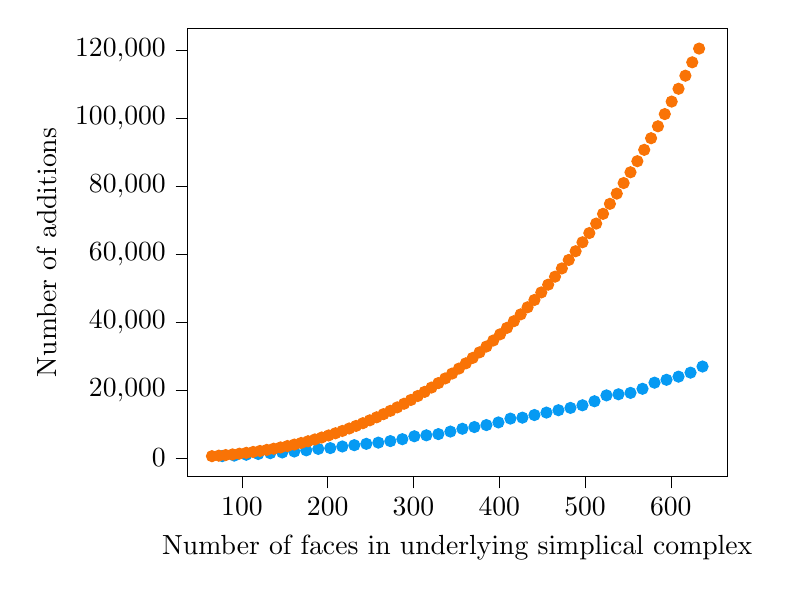
\begin{tikzpicture}
\definecolor{color0}{rgb}{0.0235294117647059,0.603921568627451,0.952941176470588}
\definecolor{color1}{rgb}{0.976470588235294,0.450980392156863,0.0235294117647059}

\begin{axis}[
xlabel = Number of faces in underlying simplical complex,
tick align=outside,
tick pos=left,
x grid style={white!69.0196078431373!black},
xmin=36.4, xmax=665.6,
xtick style={color=black},
ylabel = Number of additions,
y grid style={white!69.0196078431373!black},
ymin=-5447.05, ymax=126620.05,
ytick style={color=black},
yticklabel style={
        /pgf/number format/fixed,
        /pgf/number format/precision=5
},
scaled y ticks=false
]
\addplot [only marks, mark=*, draw=color0, fill=color0, colormap/viridis]
table{%
x                      y
77 569
91 723
105 980
119 1203
133 1439
147 1651
161 1930
175 2273
189 2694
203 2931
217 3408
231 3792
245 4184
259 4544
273 4994
287 5559
301 6417
315 6696
329 7053
343 7798
357 8627
371 9133
385 9713
399 10495
413 11620
427 11901
441 12674
455 13391
469 14095
483 14775
497 15544
511 16727
525 18461
539 18782
553 19196
567 20405
581 22205
595 23053
609 23980
623 25158
637 26965
};
\addplot [only marks, mark=*, draw=color1, fill=color1, colormap/viridis]
table{%
x                      y
65 556
73 707
81 879
89 1073
97 1290
105 1531
113 1797
121 2089
129 2408
137 2755
145 3131
153 3537
161 3974
169 4443
177 4945
185 5481
193 6052
201 6659
209 7303
217 7985
225 8706
233 9467
241 10269
249 11113
257 12000
265 12931
273 13907
281 14929
289 15998
297 17115
305 18281
313 19497
321 20764
329 22083
337 23455
345 24881
353 26362
361 27899
369 29493
377 31145
385 32856
393 34627
401 36459
409 38353
417 40310
425 42331
433 44417
441 46569
449 48788
457 51075
465 53431
473 55857
481 58354
489 60923
497 63565
505 66281
513 69072
521 71939
529 74883
537 77905
545 81006
553 84187
561 87449
569 90793
577 94220
585 97731
593 101327
601 105009
609 108778
617 112635
625 116581
633 120617
};
\end{axis}

\end{tikzpicture}

\caption{Comparision of the two constructions that yield cubical running time. Construction by Dimitriy Morozov in blue and the one propsed in this section in orange.}
\label{fig:compare}
\end{figure}
As we can see the construction propsed here grows much faster. As we have previously discussed the number of vertices, edges and triangles of the $n$-gon with fins depends on $n$. To be precise the $f$-vector of the construction is $(1+2n,4n,2n)$, i.e. all entries depend linearly on $n$, in particular all entries depend linearly on the number of vertices. For the construction of Dimitriy Morozov it also holds that the number of edges and triangles depends linearly on the number of vertices. 

Python code, to generate the filtrations of both constructions can be found on \href{https://github.com/IvanSpirandelli/Masterarbeit/blob/master/Examples/worst_case_examples.py}{[GitHub]}, see also \cite{github}. 

When considering the $n$-gon construction in terms of Theorem \ref{thm:vpath_delta} we see that for the reduction of fin triangles we follow $V$-paths defined by the apparent pairs of base triangles and base edges. Indeed, we do not get equality since the final reduction step always corresponds to an addition of the first fin triangle, which is unpaired with respect to the apparent gradient.

The lower bound we get by Theorem \ref{thm:vpath_delta} equals $\sum_{r=1}^{n-1} r = \frac{(n-1)n}{2}$ which is not the exact number of column additions but at least asymptotically correct. 

However we can generate an almost identical filtration by reversing the order of the base edges which by the same reasoning results in the same asymptotic bound of additions but has a single apparent pair. In this case the bound we get by Theorem \ref{thm:vpath_delta} is as bad as asymptotically possible.

\section{Conclusions}
The initial question that motivated this chapter was how complicated discrete Morse functions correspond to difficult persistent homology computations. While we can not give a complete answer to this we have shed some light on the relation between filtrations and gradient vector fields. We have proven a new theorem (Theorem \ref{thm:vpath_delta}), which states how the apparent gradients give a lower bound on the complexity of persistent homology computations. On the other hand we have also seen that two different filtrations of the same simplicial complex can yield an asymptotically perfect bound or a trivial constant bound that has an arbitrarily large difference to the actual number of column additions. Nevertheless, we hope that the results we discussed here prove fruitful for future research on the topic.
